

%% ══════════════════════════════════════════════════════════════════════════════
%% PART 5: QUESTIONNAIRE SLIDES (2 SLIDES)
%% ══════════════════════════════════════════════════════════════════════════════

\begin{frame}{Measuring Presence and Usability in XR}
	\textbf{\textcolor{gbAqua}{Presence Measurement: IGroup Presence Questionnaire (IPQ)}}
	
	\begin{itemize}
		\item 14 items, 7-point Likert scale
		\item Three subscales: Spatial Presence, Involvement, Realism
		\item Additional general ``being there'' item
		\item Widely validated across immersive and non-immersive contexts
	\end{itemize}
	
	\vspace{0.3cm}
	
	\textbf{\textcolor{gbAqua}{Usability Measurement: SUS for Kids}}
	
	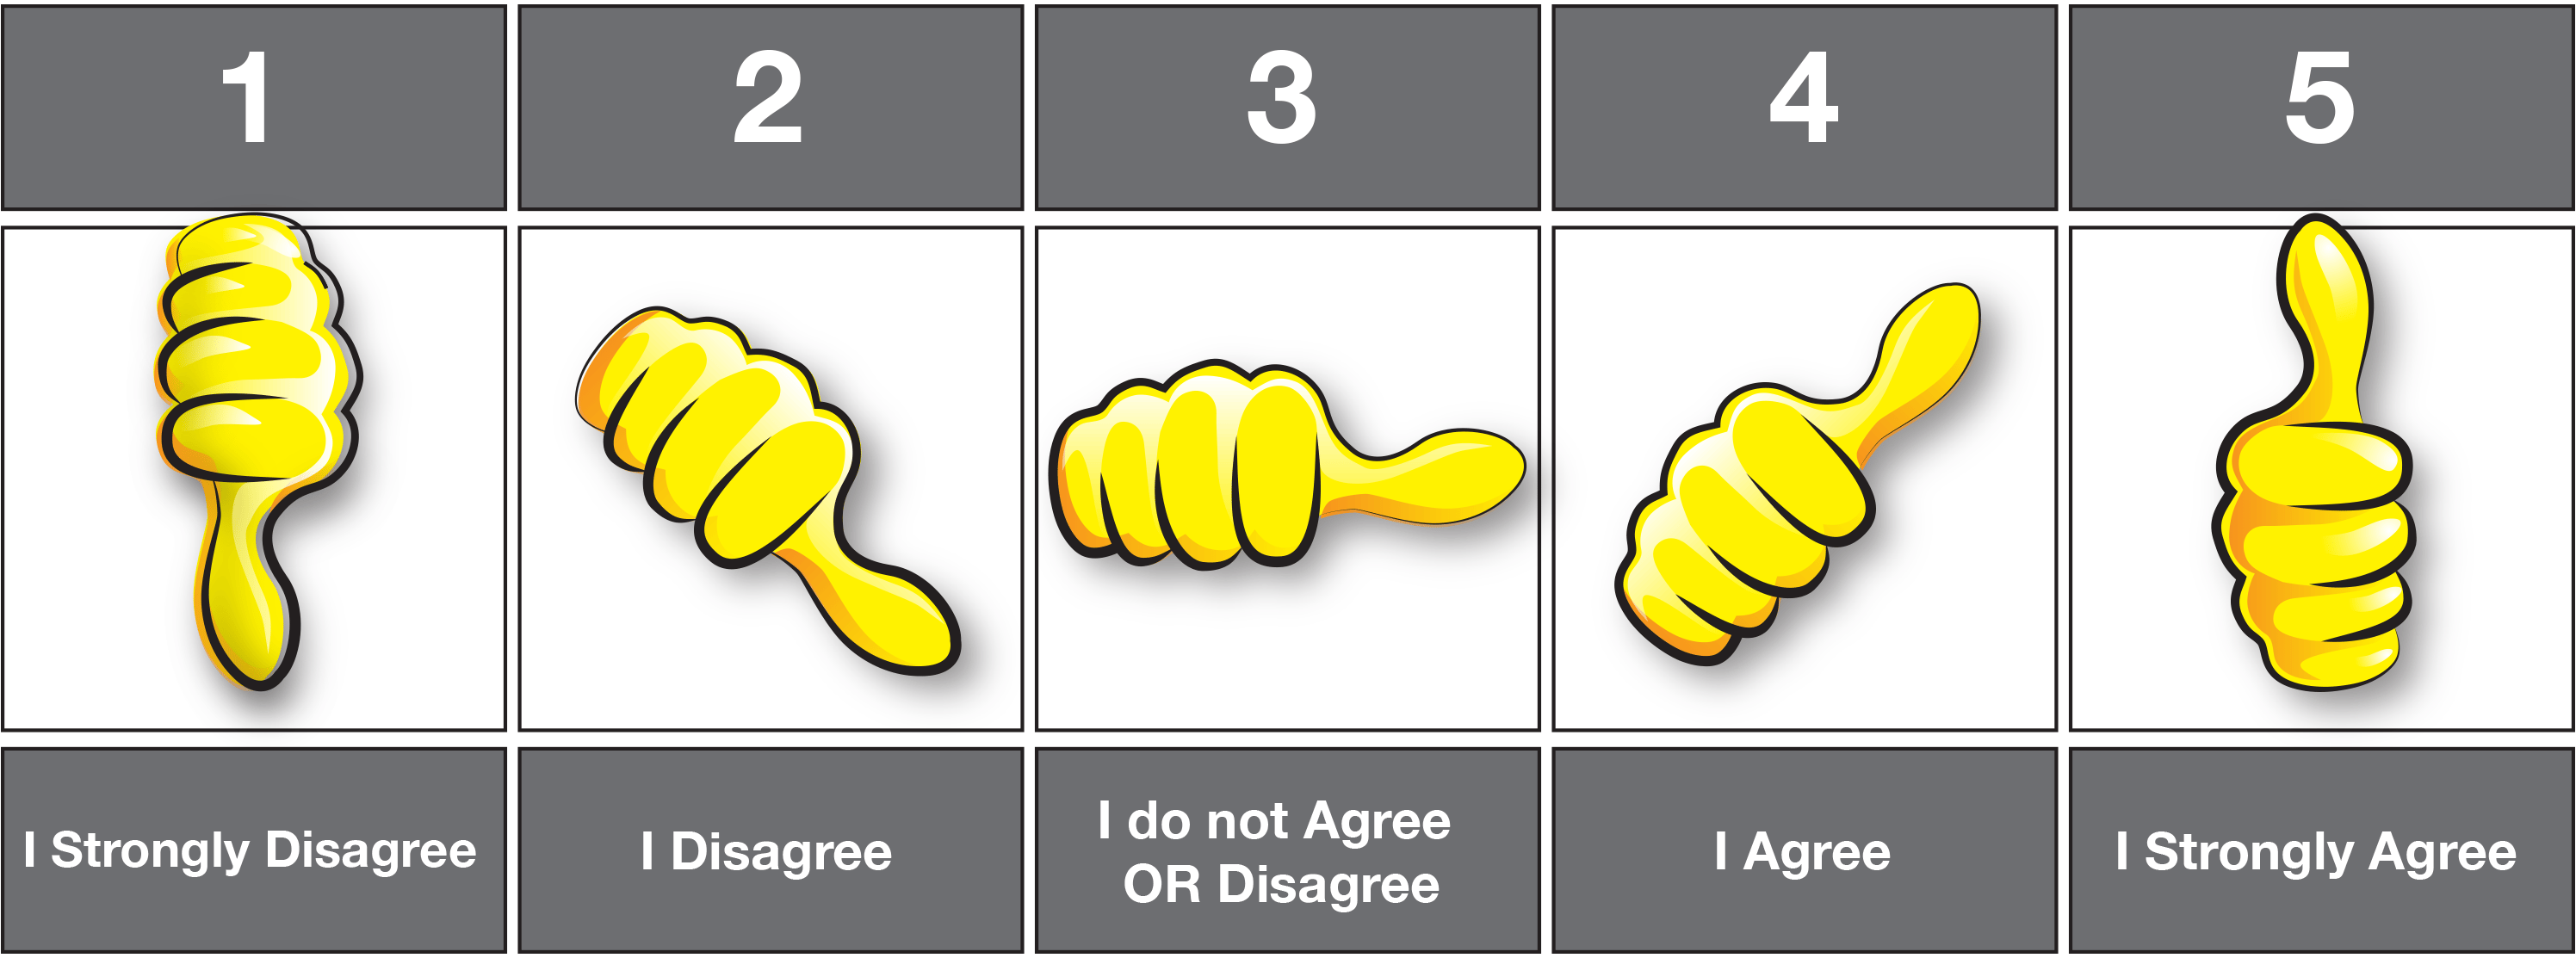
\includegraphics[width=0.8\columnwidth]{figures/SUSkids.png}
	
	\small Adapted for children ages 7-11: simplified language (grade 2-4 level), visual 5-point Likert with emoji thumbs, three additional enjoyment items.
	
	\citefooter{Schubert et al., 2001; Putnam et al., 2020}
\end{frame}

\begin{frame}{Measuring Cognitive Load and Engagement}
	\textbf{\textcolor{gbAqua}{Cognitive Load: NASA Raw Task Load Index (RTLX)}}
	
	\begin{itemize}
		\item 6 dimensions: Mental Demand, Physical Demand, Temporal Demand, Performance, Effort, Frustration
		\item Each rated on 100-point scale
		\item Faster to administer than standard NASA-TLX
		\item Maintains sensitivity to workload differences
	\end{itemize}
	
	\vspace{0.3cm}
	
	\textbf{\textcolor{gbAqua}{Engagement: User Engagement Scale Short Form (UES-SF)}}
	
	\begin{itemize}
		\item 12 items, 5-point Likert scale
		\item Four dimensions:
		\begin{itemize}
			\item Focused Attention: Absorbed in experience
			\item Perceived Usability: Ease of use
			\item Aesthetic Appeal: Visual attractiveness
			\item Reward Factor: Sense of valued outcome
		\end{itemize}
	\end{itemize}
	
	\citefooter{Hart \& Staveland, 1988; O'Brien et al., 2018}
\end{frame}
